% THIS IS AN EXAMPLE DOCUMENT FOR VLDB 2012
% based on ACM SIGPROC-SP.TEX VERSION 2.7
% Modified by  Gerald Weber <gerald@cs.auckland.ac.nz>
% Removed the requirement to include *bbl file in here. (AhmetSacan, Sep2012)
% Fixed the equation on page 3 to prevent line overflow. (AhmetSacan, Sep2012)


\documentclass{vldb}
\usepackage{graphicx}
\usepackage{pgfplots}
\usepackage{balance}  % for  \balance command ON LAST PAGE  (only there!)
\usepackage{array}

% smart quotes
\usepackage [autostyle, english = american]{csquotes}
\MakeOuterQuote{"}

% Include information below and uncomment for camera ready
\vldbTitle{TLA+ Trace Checking In Production}
\vldbAuthors{A. Jesse Jiryu Davis, Max Hirschhorn, Judah Schvimer}
\vldbDOI{https://doi.org/10.14778/xxxxxxx.xxxxxxx}
\vldbVolume{12}
\vldbNumber{xxx}
\vldbYear{2020}

\begin{document}

% ****************** TITLE ****************************************

\title{Model-Based Testing in Practice}
% OUTLINE: https://docs.google.com/document/d/16qDw3hxpi64ASPm0j0HneQSjyY7Kf93tCCLzG1NdOFM/edit

% possible, but not really needed or used for PVLDB:
%\subtitle{[Extended Abstract]
%\titlenote{A full version of this paper is available as\textit{Author's Guide to Preparing ACM SIG Proceedings Using \LaTeX$2_\epsilon$\ and BibTeX} at \texttt{www.acm.org/eaddress.htm}}}

% ****************** AUTHORS **************************************

% You need the command \numberofauthors to handle the 'placement
% and alignment' of the authors beneath the title.
%
% For aesthetic reasons, we recommend 'three authors at a time'
% i.e. three 'name/affiliation blocks' be placed beneath the title.
%
% NOTE: You are NOT restricted in how many 'rows' of
% "name/affiliations" may appear. We just ask that you restrict
% the number of 'columns' to three.
%
% Because of the available 'opening page real-estate'
% we ask you to refrain from putting more than six authors
% (two rows with three columns) beneath the article title.
% More than six makes the first-page appear very cluttered indeed.
%
% Use the \alignauthor commands to handle the names
% and affiliations for an 'aesthetic maximum' of six authors.
% Add names, affiliations, addresses for
% the seventh etc. author(s) as the argument for the
% \additionalauthors command.
% These 'additional authors' will be output/set for you
% without further effort on your part as the last section in
% the body of your article BEFORE References or any Appendices.

\numberofauthors{3} %  
\author{
% The command \alignauthor (no curly braces needed) should
% precede each author name, affiliation/snail-mail address and
% e-mail address. Additionally, tag each line of
% affiliation/address with \affaddr, and tag the
% e-mail address with \email.
%
% TODO: don't repeat mailing address
% 1st. author
\alignauthor
A. Jesse Jiryu Davis\\
       \affaddr{MongoDB, Inc.}\\
       \affaddr{1633 Broadway}\\
       \affaddr{New York, NY 10019}\\
       \email{jesse@mongodb.com}
% 2nd. author
\alignauthor
Max Hirschhorn\\
       \affaddr{MongoDB, Inc.}\\
       \affaddr{1633 Broadway}\\
       \affaddr{New York, NY 10019}\\
       \email{max.hirschhorn@mongodb.com}
\alignauthor
Judah Schvimer\\
       \affaddr{MongoDB, Inc.}\\
       \affaddr{1633 Broadway}\\
       \affaddr{New York, NY 10019}\\
       \email{judah@mongodb.com}
}
% There's nothing stopping you putting the seventh, eighth, etc.
% author on the opening page (as the 'third row') but we ask,
% for aesthetic reasons that you place these 'additional authors'
% in the \additional authors block, viz.

% Just remember to make sure that the TOTAL number of authors
% is the number that will appear on the first page PLUS the
% number that will appear in the \additionalauthors section.


\maketitle

% ********************************************************************
% ****************** Abstract ****************************************
% ********************************************************************
\begin{abstract}

TODO
\end{abstract}

% ********************************************************************
% ****************** Introduction ************************************
% ********************************************************************
\section{Introduction}
\label{sec:introduction}

It is well established that formal modelling catches bugs, aids software design, and improves code quality \cite{Newcombe2014UseOfFormalMethodsAmazon}.
Formal methods are increasingly being used to gain confidence in mission-critical, highly complex systems in multiple domains across many companies. 
Amazon \cite{Newcombe2014UseOfFormalMethodsAmazon, Chudnov18AmazonS2N, Cook18SecurityAWS}, Intel \cite{Kaivola09IntelI7, Beers08IntelExperience}, Microsoft \cite{Shukla18AzureCosmosDB}, and Springer Verlag \cite{Neubauer12AutomatedContinuousQualityAssurance}, have all written about their uses of formal methods and the value they've gained from modelling and verifying industrial software. 
But software engineers in industry are often skeptical of the value of the model unless it can be shown to match the implementation \cite{Wayne18AgileFormalMethods, Newcombe2014UseOfFormalMethodsAmazon}, due to the risk of \textit{transcription bugs}.
Further, it can be difficult to ensure that in a large engineering organization, changes in the production code are accompanied by changes in the model of the code.
"eXtreme Modelling", in which "model and implementation are developed in parallel" \cite{Gravell11ConcurrentDevelopmentOfModelAndImplementation}, has been proposed as a solution to spec and implementation divergence.

We made two different attempts to put "eXtreme Modelling's" findings into production.
"eXtreme Modelling" proposes the following guidelines for ensuring spec and implementation conformance:
\begin{enumerate}
  \item Model is written immediately prior to implementation
  \item Model checkers verify the model meets certain properties
  \item Multiple models are produced for different aspects of the system
  \item Models generate tests, add assertions in code, and trace checkers verify that test traces are legal in the model
  \item Models evolve with the implementation
  \item Continuous integration verifies the model and its conformance to the implementation with every code change
\end{enumerate}

Although "eXtreme Modelling" was not intended for existing code bases and models, we attempted to lay the groundwork to use this technique on future projects in which we would write the model before the implementation, and future code changes could affect the code's conformance with its model.

\subsection{Contributions}

We undertook two case studies, using two existing code bases.
In the MongoDB Server, we attempted model-based trace-checking (MBTC). 
One of the requirements was that implementing MBTC for future models should be cheap, following an initial investment in infrastructure.
After a great deal of effort, we determined that future models would not be easily trace-checked, and decided MBTC was impractical for the MongoDB Server, largely due to the system's enormous size and complex internal concurrency control.
In MongoDB Realm Sync, we succeeded in using model-based test-case generation (MBTCG), to ensure conformance between a spec, and multiple implementations of that spec in different programming languages.

This paper will show what factors made MBTCG successful and MBTC unsuccessful, and attempt to answer the questions, "When should I attempt MBTC?" and "When should I attempt MBTCG?".
This paper will identify lessons learned in both techniques and avenues of future research to make MBTC more practical.

This paper provides background to this research in Section \ref{sec:background}. 
Section \ref{sec:related_work} reviews related work. 
Section \ref{sec:model_based_trace_checking} describes our attempt at MBTC, and the challenges met. 
\ref{sec:model_based_test_case_generation} describes our success with MBTCG. 
Finally, Section \ref{sec:conclusions} details our conclusions and avenues for future work.

% ********************************************************************
% ****************** Background **************************************
% ********************************************************************
\section{Background}
\label{sec:background}

\subsection{MongoDB Server}
\label{subsec:background_server}

The MongoDB Server is a distributed document database with features that are traditionally found both in NoSQL and Relational DBMSes.
It has support for flexible unstructured schemas, as well as ACID compliant transactions and secondary indexes \cite{Kamsky19TPCCMongoDB}.
MongoDB Servers are typically deployed as a redundant group called a "replica set", which uses a protocol inspired by Raft \cite{Ongaro14Raft} to elect a leader node and replicate data changes to follower nodes.
Each node maintains a copy of the data and a durable log of operations, the "oplog".
Reads and writes offer multiple consistency and durability levels with increasingly strong guarantees \cite{Schultz19TunableConsistency, Tyulenev19CausalConsistencyMongoDB}.
The MongoDB Server has been under open-source development for 12 years, with hundreds of thousands of lines of code, and dozens of active contributors at any time.

\subsection{MongoDB Realm Sync}
\label{subsec:background_realm}

MongoDB Realm is an offline-first database with a full-duplex synchronization protocol; the client is able to  upload new changes to the server without needing to download new changes from the server.

TODO (Max): Mention "automatic conflict resolution" being handled by an operational transformation algorithm
TODO (Max): Explain what operational transformation is (cite some paper)
TODO (Max): Ensure the word "merge" is used to describe when two peers exchange changes that have occurred on their branch of history since their common point. Unclear at this point if we should describe as being similar to git or not. It is likely necessary to describe how clients keep an immutable history and so subsequent changes are ``rebased'' by being appended to the end of that history.
TODO (Max): For changesets that are based on the same version of history (think git-merge-base) the order in which they occur relative to each other is the (timestamp, client id) of the changeset. The model explicitly chose not to represent time so client id becomes the only time-ordering mechanic the merge rules care about.

To ensure both Realm and the MongoDB Server provide advertised consistency guarantees with good performance, we run thousands of correctness and performance tests in Evergreen, our continuous integration (CI) system \cite{Daly19iChangePointMongoDB}.
These tests rely heavily on randomized testing, both randomly changing the topology and running randomized commands \cite{Guo17MongoDBFuzzTester}.
Randomized tests provided an abundant set of traces to consider using for MBTC.

\subsection{TLA+ and TLC}
\label{subsec:background_tla_tlc}

To gain the benefits of formal methods, engineers on MongoDB's Server-Replication Team wrote models to verify several concurrent and distributed protocols in the Server \cite{Schultz19BugsLife}.
The formal modelling language we chose, TLA+, was introduced by Leslie Lamport in 1999 \cite{Lamport99TLAPlus, Lamport02SpecifyingSystems}.
A TLA+ model defines a set of variables expressing a system's state, and the actions which may modify this state.
The model may include simple invariants that must hold at each moment, as well as \textit{temporal logic} formulas to express properties of the system's execution over time.
TLA+ is a precise mathematical language; thus the properties of a TLA+ model can be proven correct, or validated by a finite model-checker which exhaustively explores its behaviors.
The standard model-checker for TLA+, TLC, is actively developed on GitHub \cite{TLAPlusGitHub}.
MongoDB chose TLA+ due to its success in industry and academic distributed systems research, open source implementation, and rich tooling.

Prior to this work, we had TLA+ models for the MongoDB Server's replication protocol, its initial sync protocol, and some aspects of its hierarchical locking rules.
Concurrently with this work, other engineers wrote models for a new replica set reconfiguration protocol and a proposed but rejected reconfiguration protocol.
In concert with this work, we created the Realm Operational Transformation model.
Models for future features and existing distributed protocols are currently planned for development.
Models are written to gain confidence in critical aspects of our system, and then code reviewed and committed to the same repository as our tests and code using the same process as we use for our tests and code.
Engineering work is scheduled to continuously verify our models alongside our correctness tests, to ensure that any changes to our models are correctly verified, and to document what model configuration was used to verify them.

\subsection{MBTC and MBTCG}
\label{subsec:background_mbtc_mbt}

The "eXtreme Modelling" approach includes two testing methods that are promising for MongoDB: model-based trace-checking (MBTC) \cite{Jard83AnApproachToTestingSpecifications, MBTC} and model-based test-case generation (MBTCG) \cite{Utting06PracticalModelBasedTesting}. 

In MBTC, the implementation under test (IUT) is exercised with a test or by observing its behavior in production.
The IUT produces an execution trace that captures its sequence of state changes.
This execution trace is checked against the model, either while the IUT is running or post-hoc, to verify that the trace is a permitted behavior of the model.
The greater the variety of observed behaviors, the more confidence one has in the implementation's conformance.

In MBTCG, the model is used to generate test inputs and expected outputs, either exhaustively or from a carefully selected subset \cite{Dick93AutomatingGenerationOfTests}.
A test framework provides the generated inputs to the IUT and checks whether it responds as specified.


% ********************************************************************
% ****************** Related Work ************************************
% ********************************************************************
\section{Related Work}
\label{sec:related_work}

% TODO: jesse, add MBTCG references

Our work builds primarily on the "eXtreme Modelling" approach proposed by Gravell, et. al. \cite{Gravell11ConcurrentDevelopmentOfModelAndImplementation}, and closely related work by Augusto, et. al.\cite{Augusto03ValidatingBusinessSystems}. 
In these papers, the authors discuss the co-evolution of two e-business applications implemented in Java with several small models written in Promela and B.
They describe specification engineering techniques; for example, holding regular meetings between modellers and implementers, and maintaining a dictionary to translate between names in the model and the implementation.
Such techniques seem promising, but the authors analyze their effectiveness when practiced on an example application developed by a team of four academics, not on commercial software developed by hundreds of engineers.
We have attempted to put the ideas of "eXtreme Modelling" into practice with complex commercial software instead of a research prototype, and using TLA+ and C++ instead of Java, B, and Promela.
To our knowledge, no prior research demonstrates all characteristics of "eXtreme Modelling" in industry.

A variety of other methods have been proposed to ensure that an implementation conforms to its formal models.
Some projects use the same language for spec and implementation \cite{KerGre99}, some generate implementation code from the spec \cite{Houhou17CodeGenerationFromSpecification}, others apply model-checking or formal verification directly to the implementation \cite{Holzmann04ModelDrivenVerification, Chudnov18ContinuousFormalVerification}, and yet others perform verified step-wise refinement from the high-level spec all the way down to the implementation \cite{Eiriksson95UsingFormalVerification}.
Any of these methods provides high confidence that the implementation conforms (although even a verified system is not bug-free \cite{Fonseca17EmpiricalStudy}). 
However, these methods cannot be used with our system, MongoDB.
In the research we have reviewed, they are limited to small programs, either written in C or a specialized language such as Prolog; they have not been demonstrated with our implementation language, C++, nor on very large software systems such as ours, which is over 700,000 executable lines of code.
They also cannot be used when writing new models for a system that has already been implemented.

Ural et. al. in \cite{Ural84AutomatedTestingOfProtocolSpecifications} propose to begin with a high-level specification and refine it in stages, using MBTC to gain confidence that each stage's model is equivalent to the previous stage.
This technique is incompatible with "eXtreme Modelling": multiple high-level specifications cannot describe a single system, and co-evolution of model and implementation is not practical with this technique, because one would have to repeat the effort of step-wise refinement from top to bottom with each change.

Tasiran et. al. \cite{Tasiran03AlphaMicroprocessor} implement MBTC to check that a simulated microprocessor's behavior conforms to its TLA+ specification.
After each simulation step they invoke the TLC model-checker to determine if the step is permitted by the specification.
The authors describe a sophisticated method to measure their tests' coverage of the specification's state space: they first eliminate symmetrical states, and project to a smaller space with a view function, before comparing to the covered space.

Neubauer et. al. in \cite{Neubauer12AutomatedContinuousQualityAssurance} use machine learning to infer a formal model of a commercial software system from its observed behaviors.
They use MBTC to check if later execution traces of the system still conform to the inferred model; if not, either the system has a bug or the system behaved correctly and the model must be updated.
This work approaches the "eXtreme Modelling" development style, but an inferred model is quite different from one written by humans; the purpose of the former is solely to detect behavior changes in the implementation, the latter expresses the designers' intent.

% ********************************************************************
% ****************** MBTC ********************************************
% ********************************************************************
\section{Model-Based Trace-Checking}
\label{sec:model_based_trace_checking}

TODO: This case-study content can be cut, or merged with the below section.
\subsection{Case Study: MongoDB Server}
The MongoDB engineering team has used TLA+ to model several aspects of the MongoDB Server prior to this paper's research.
The MongoDB Server's replication protocol has especially benefited from TLA+.
TLA+ has helped us design a complex, novel reconfiguration protocol, reproduce and fix multiple bugs, and verify liveness properties of the database \cite{Schultz19BugsLife}.

We attempted to use model-based trace-checking (MBTC) \cite{MBTC} to gain confidence that the C++ implementation of the database's replication system matches multiple TLA+ models.
Our proposed testing method would apply MBTC to execution traces obtained from our existing tests, and we would deploy our testing system to a cluster of continuous integration servers.
This would permit us to rapidly develop both the models and the implementation, while receiving quick feedback about divergences between the two \cite{Gravell11ConcurrentDevelopmentOfModelAndImplementation}.
***** END Case Study: MongoDB Server ****


% Each replica in a MongoDB replica set stores:

% \begin{enumerate}
% \item A log of all operations (the "oplog")
% \item A term counter that is incremented each election
% \item A (timestamp, term) pair representing the newest operation it knows has been committed by a majority of replicas (the "commit point")
% \end{enumerate}

MongoDB's Server-Replication Team has written several TLA+ models to describe aspects of the MongoDB Server, and even different aspects of the core replication protocol. 
Our goal was to test that a replica set's actual behavior conforms to these models.

\subsection{Implementing MBTC}
\label{subsec:mbtc_solution}

\begin{figure}
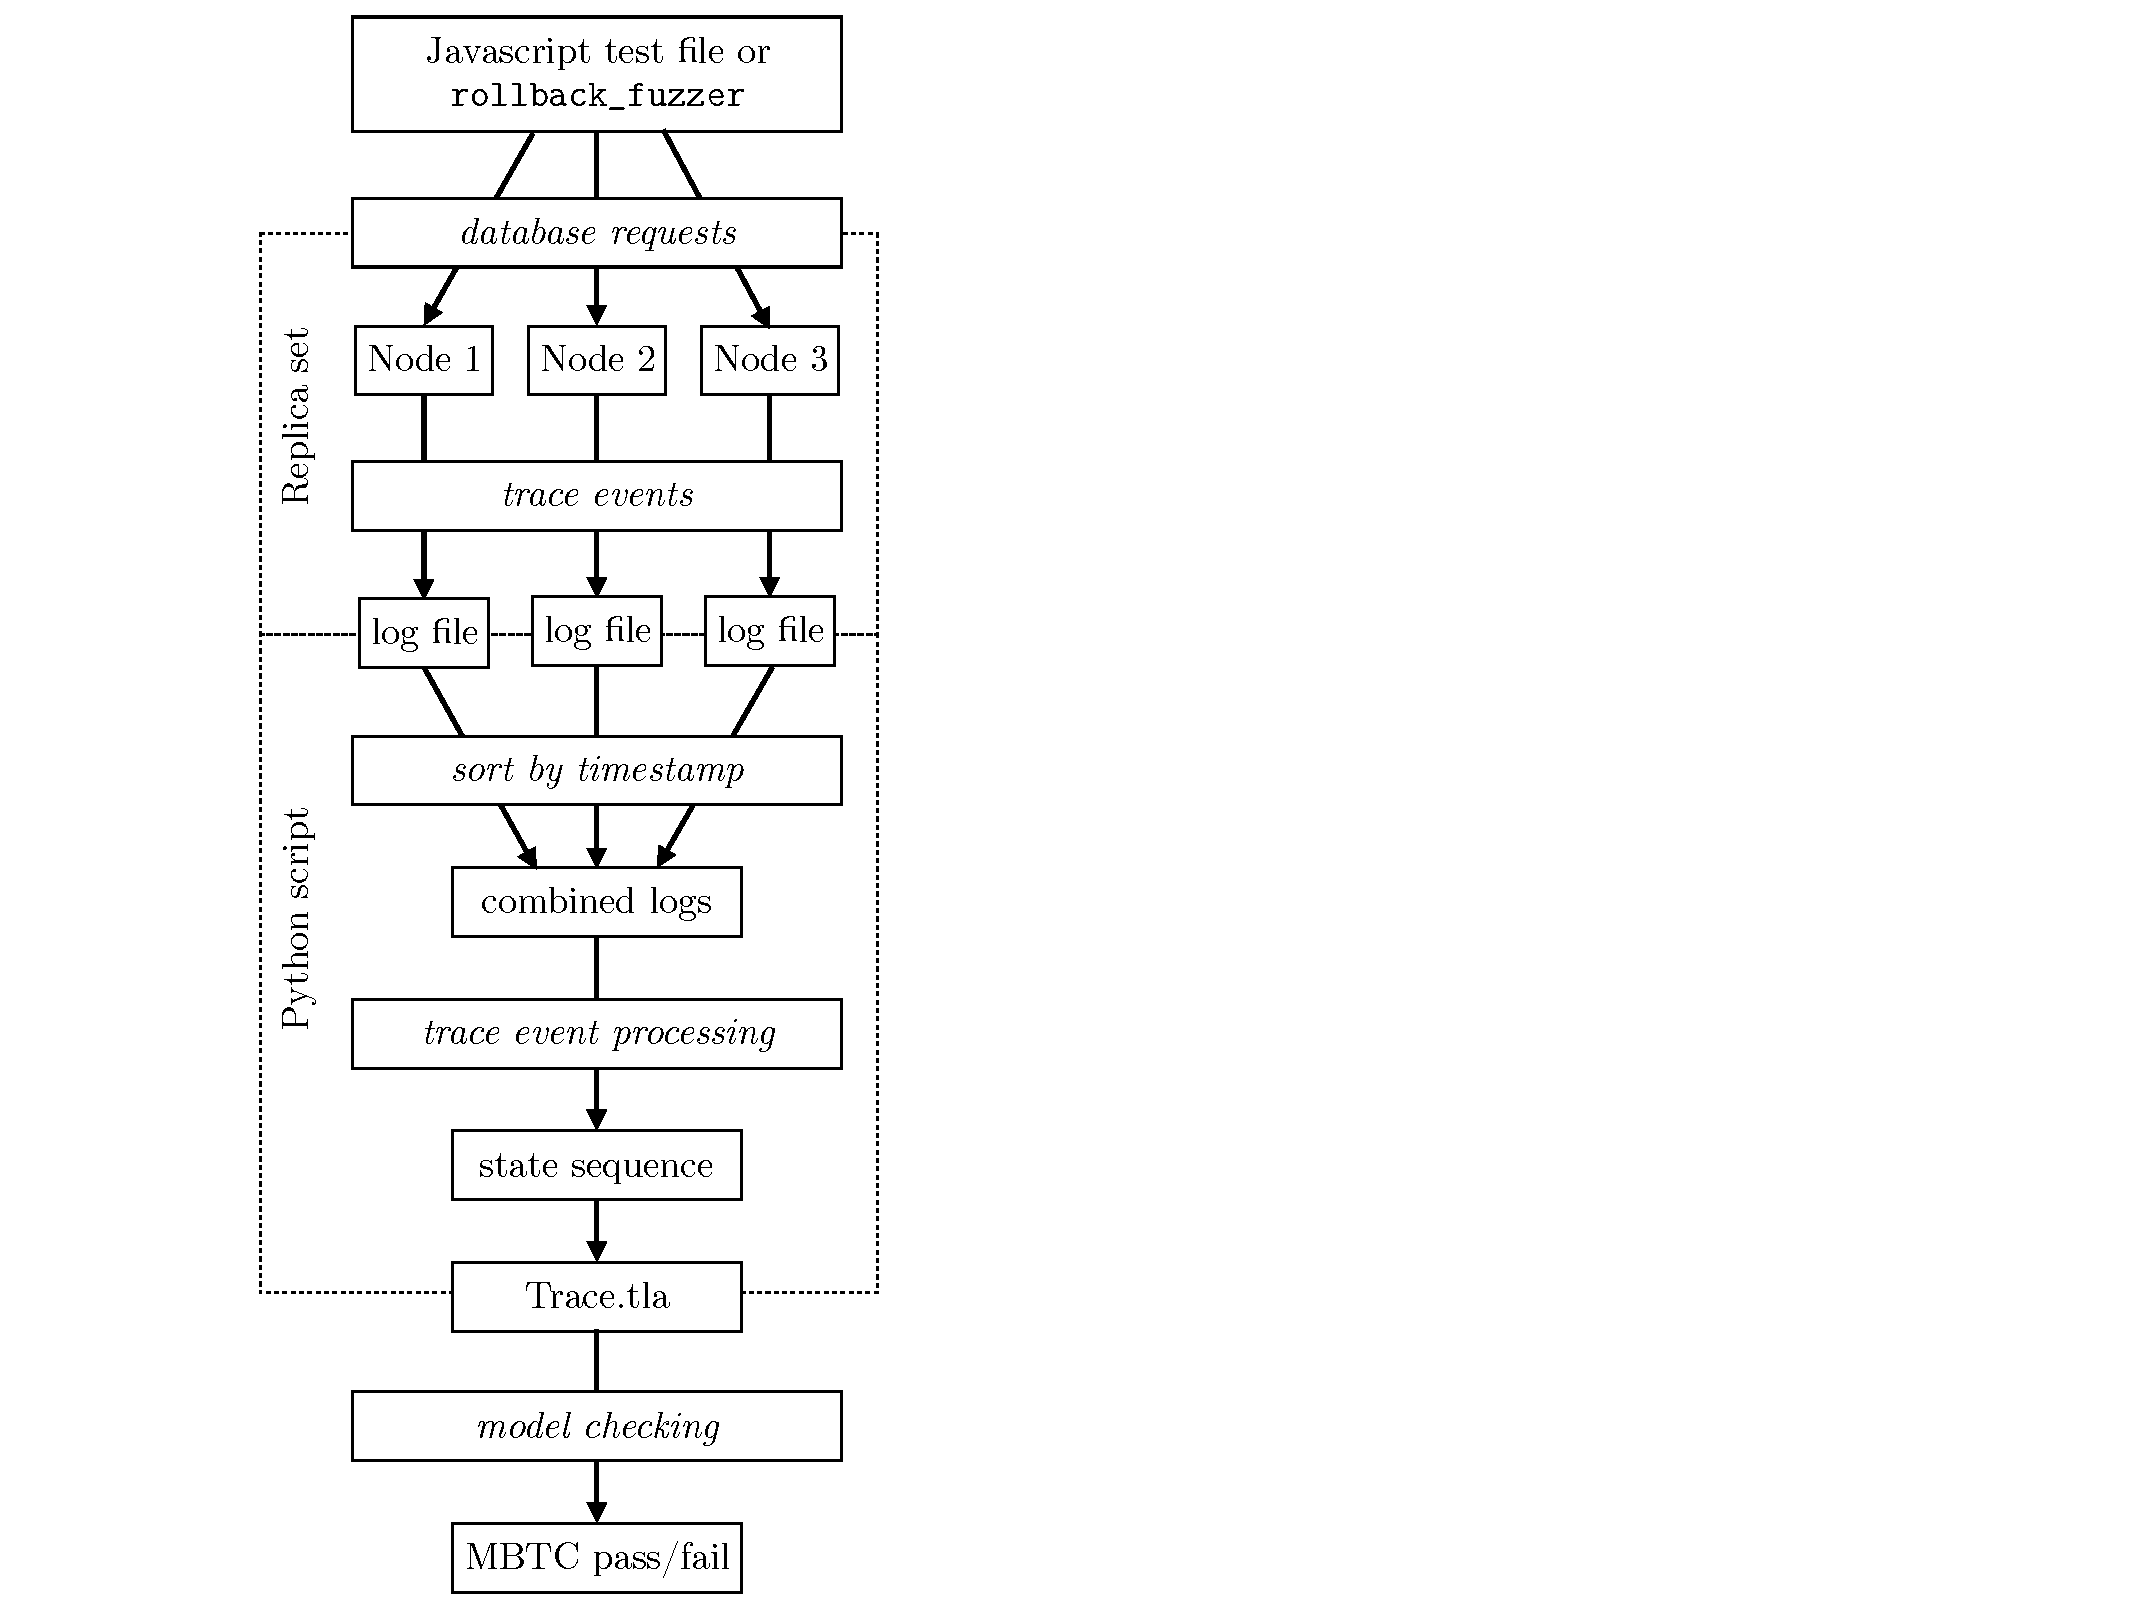
\includegraphics[width=\textwidth]{MBTC-pipeline.pdf}
\caption{MBTC data pipeline}
\label{figure:MBTC-pipline}
\end{figure}

Prior to our research, there were 423 integration tests handwritten in Javascript that exercise our replication protocol, and 23 randomized test suites that pause, disconnect, and terminate servers while the replica set is performing regular operations. 
We wanted to run these tests with additional tracing and use MBTC to check if the traces conform to our models.

For our prototype we chose one model, a 345-line TLA+ file called \texttt{RaftMongo.tla} in the MongoDB Server repository \cite{MongoGitHub}, which models the gossiping of the commit point among replicas.
This model is based on Diego Ongaro's TLA+ specification for Raft \cite{Ongaro14TLA+Raft}, with several key modifications.
One difference is that the MongoDB Server's replication protocol is a pull protocol whereas Raft is a push protocol; the MongoDB Server's follower nodes request oplog entries from the leader or other nodes, rather than the leader sending entries to followers.
\texttt{RaftMongo.tla} is very high-level with few state variables and invariants in order to focus on commit point propagation. Unlike Ongaro's work, our specification does not explicitly model messages passed between nodes.

Each replica's state is modeled with four variables:

\begin{description}
\item \texttt{role}: "Leader" or "Follower"
\item \texttt{term}: Newest election term the replica knows
\item \texttt{commitPoint}: Newest majority-committed timestamp it knows
\item \texttt{oplog}: Contents of its oplog
\end{description}

There are seven named state transitions in the model:

\begin{description}
\item \texttt{AppendOplog}: A node receives entries from any node
\item \texttt{RollbackOplog}: A node removes divergent entries
\item \texttt{BecomePrimaryByMagic}: A node is elected leader "by magic"---the election protocol is not modeled
\item \texttt{Stepdown}: A leader becomes a follower
\item \texttt{ClientWrite}: A leader executes write operations
\item \texttt{AdvanceCommitPoint}: The leader advances the commit point
\item \texttt{UpdateTermThroughHeartbeat}: A node learns the election term from any node
\item \texttt{LearnCommitPointWithTermCheck}: A node learns the commit point from any node
\item \texttt{LearnCommitPointFromSyncSourceNeverBeyondLast-\linebreak{}Applied}: A node learns the commit point from a more up-to-date node
\end{description}

When we configure this model with 3 replicas and constrain the model-checker to at most 3 terms and oplogs up to 3 entries long, TLC successfully model-checks it and discovers 371,368 distinct states.
TLC validates an invariant that committed writes are not rolled back and a temporal property that the commit point is eventually propagated.

% Reverting logging in commit bcae9e67774088 made 617 deletions,
% minus 42 are JS, 5 are SCons, leaves 570 C++
We wrote a C++ procedure \texttt{logTlaPlusTraceEvent}, enabled only in testing, which used our logging framework to emit as JSON the values of the four state variables above.
Then we located code paths in the MongoDB Server corresponding to the seven state transitions and added calls to this procedure.
The code changes required 570 lines of C++.

MBTC with a distributed system requires a partial order of trace events; we achieved a strict order by running all processes on one machine and sleeping before logging the trace event.
Since all log messages include the current timestamp with millisecond precision, it was sufficient to sleep until the system clock's millisecond digit changed (Figure \ref{fig:millisecond_sleep}.

\begin{figure}
\begin{verbatim}
PROCEDURE logTlaPlusTraceEvent() {
    /* Timestamp has millisecond precision */
    timestamp beforeTime = getCurrentTimestamp()
    timestamp afterTime = getCurrentTimestamp()
    while (afterTime == beforeTime) {
        sleep 1 millisecond
        afterTime = getCurrentTimestamp()
    }

    assert(afterTime > beforeTime, "Clock went backwards")
    log trace event and current timestamp
}
\end{verbatim}
\caption{Pseudocode for logTlaPlusTraceEvent}
\label{fig:millisecond_sleep}
\end{figure}

(Jard et. al. describe a solution with vector clocks \cite{Jard94GeneralApproachToTraceChecking}.)

% Run on Jesse's workstation at commit https://github.com/ajdavis/mongo/commit/95f70b
% python3 buildscripts/resmoke.py --suites=replica_sets --storageEngine=wiredTiger --continueOnFailure --storageEngineCacheSizeGB=1 --alwaysUseLogFiles --jobs=16
% [resmoke] 2020-01-28T11:28:13.268-0500 Summary of replica_sets suite: 423 test(s) ran in 54885.49 seconds (303 succeeded, 0 were skipped, 120 failed, 0 errored)

We enabled tracing for our 423 handwritten Javascript tests. 
Of these, 120 failed due to incompatibilities with tracing. 
(We describe these incompatibilities in Section \ref{subsubsec:mbtc_impl_discrepencies}.)
In total, these tests produced 42,262 trace events. 
We also selected one of our randomized tests, called \texttt{rollback\_fuzzer}, for MBTC. 
This test orchestrates network partitions which cause replicas to temporarily diverge and then to roll back writes in order to re-synchronize when the partitions are healed.
Random CRUD and DDL operations are run against leader nodes in the set to test that, with high probability, all combinations of operations and their behavior on roll back work consistently.
Nodes are also randomly restarted to test that clean and unclean restarts during rollback procedures do not lead to data corruption.
A representative run of \texttt{rollback\_fuzzer} produced 2,683 trace events.

% How much TLA+ statement and space coverage did today's rollback_fuzzer suite hit?
% from a given run of the suite, 1 JS file, 3 nodes, 2683 trace events
% Follow instructions on https://github.com/tlaplus/tlaplus/issues/413
We wrote a 484-line Python script \cite{ReplTraceChecker} to post-process trace logs. 
The script merges the replicas' logs and sorts them by timestamp to obtain a sequence of trace events. 
Each event describes the state of only \textit{one} replica at the moment it executes a state transition.
In order to construct a sequence of states describing the \textit{entire} replica set, 
the script begins with a known initial state, combines it with the first trace event to determine the next state, and so on. 
The logic to combine a current state \ensuremath{S} with a trace event from replica node \ensuremath{N} to produce next state \ensuremath{S'} is as follows:

\begin{itemize}
\item \texttt{role}: If \ensuremath{N} had role "Leader" and now has role "Follower", its role in \ensuremath{S'} is "Follower" and the other nodes' role values are unchanged. If \ensuremath{N} is elected leader the script assumes all other nodes become followers instantly. Thus the role of \ensuremath{N} in \ensuremath{S'} is "Leader" and all others' role is "Follower".
\item \texttt{term}: The term of \ensuremath{N} in \ensuremath{S'} is replaced with the trace event's term. The other nodes' terms are unchanged.
\item \texttt{commitPoint} and \texttt{oplog}: Similar to term.
\end{itemize}

For example, in Figure \ref{figure:event-processing}, the replica set's current state has Node 1 as the leader in term 1. 
The script processes a trace event from Node 2 announcing it has become leader in term 2, arriving at the next state.

\begin{figure}
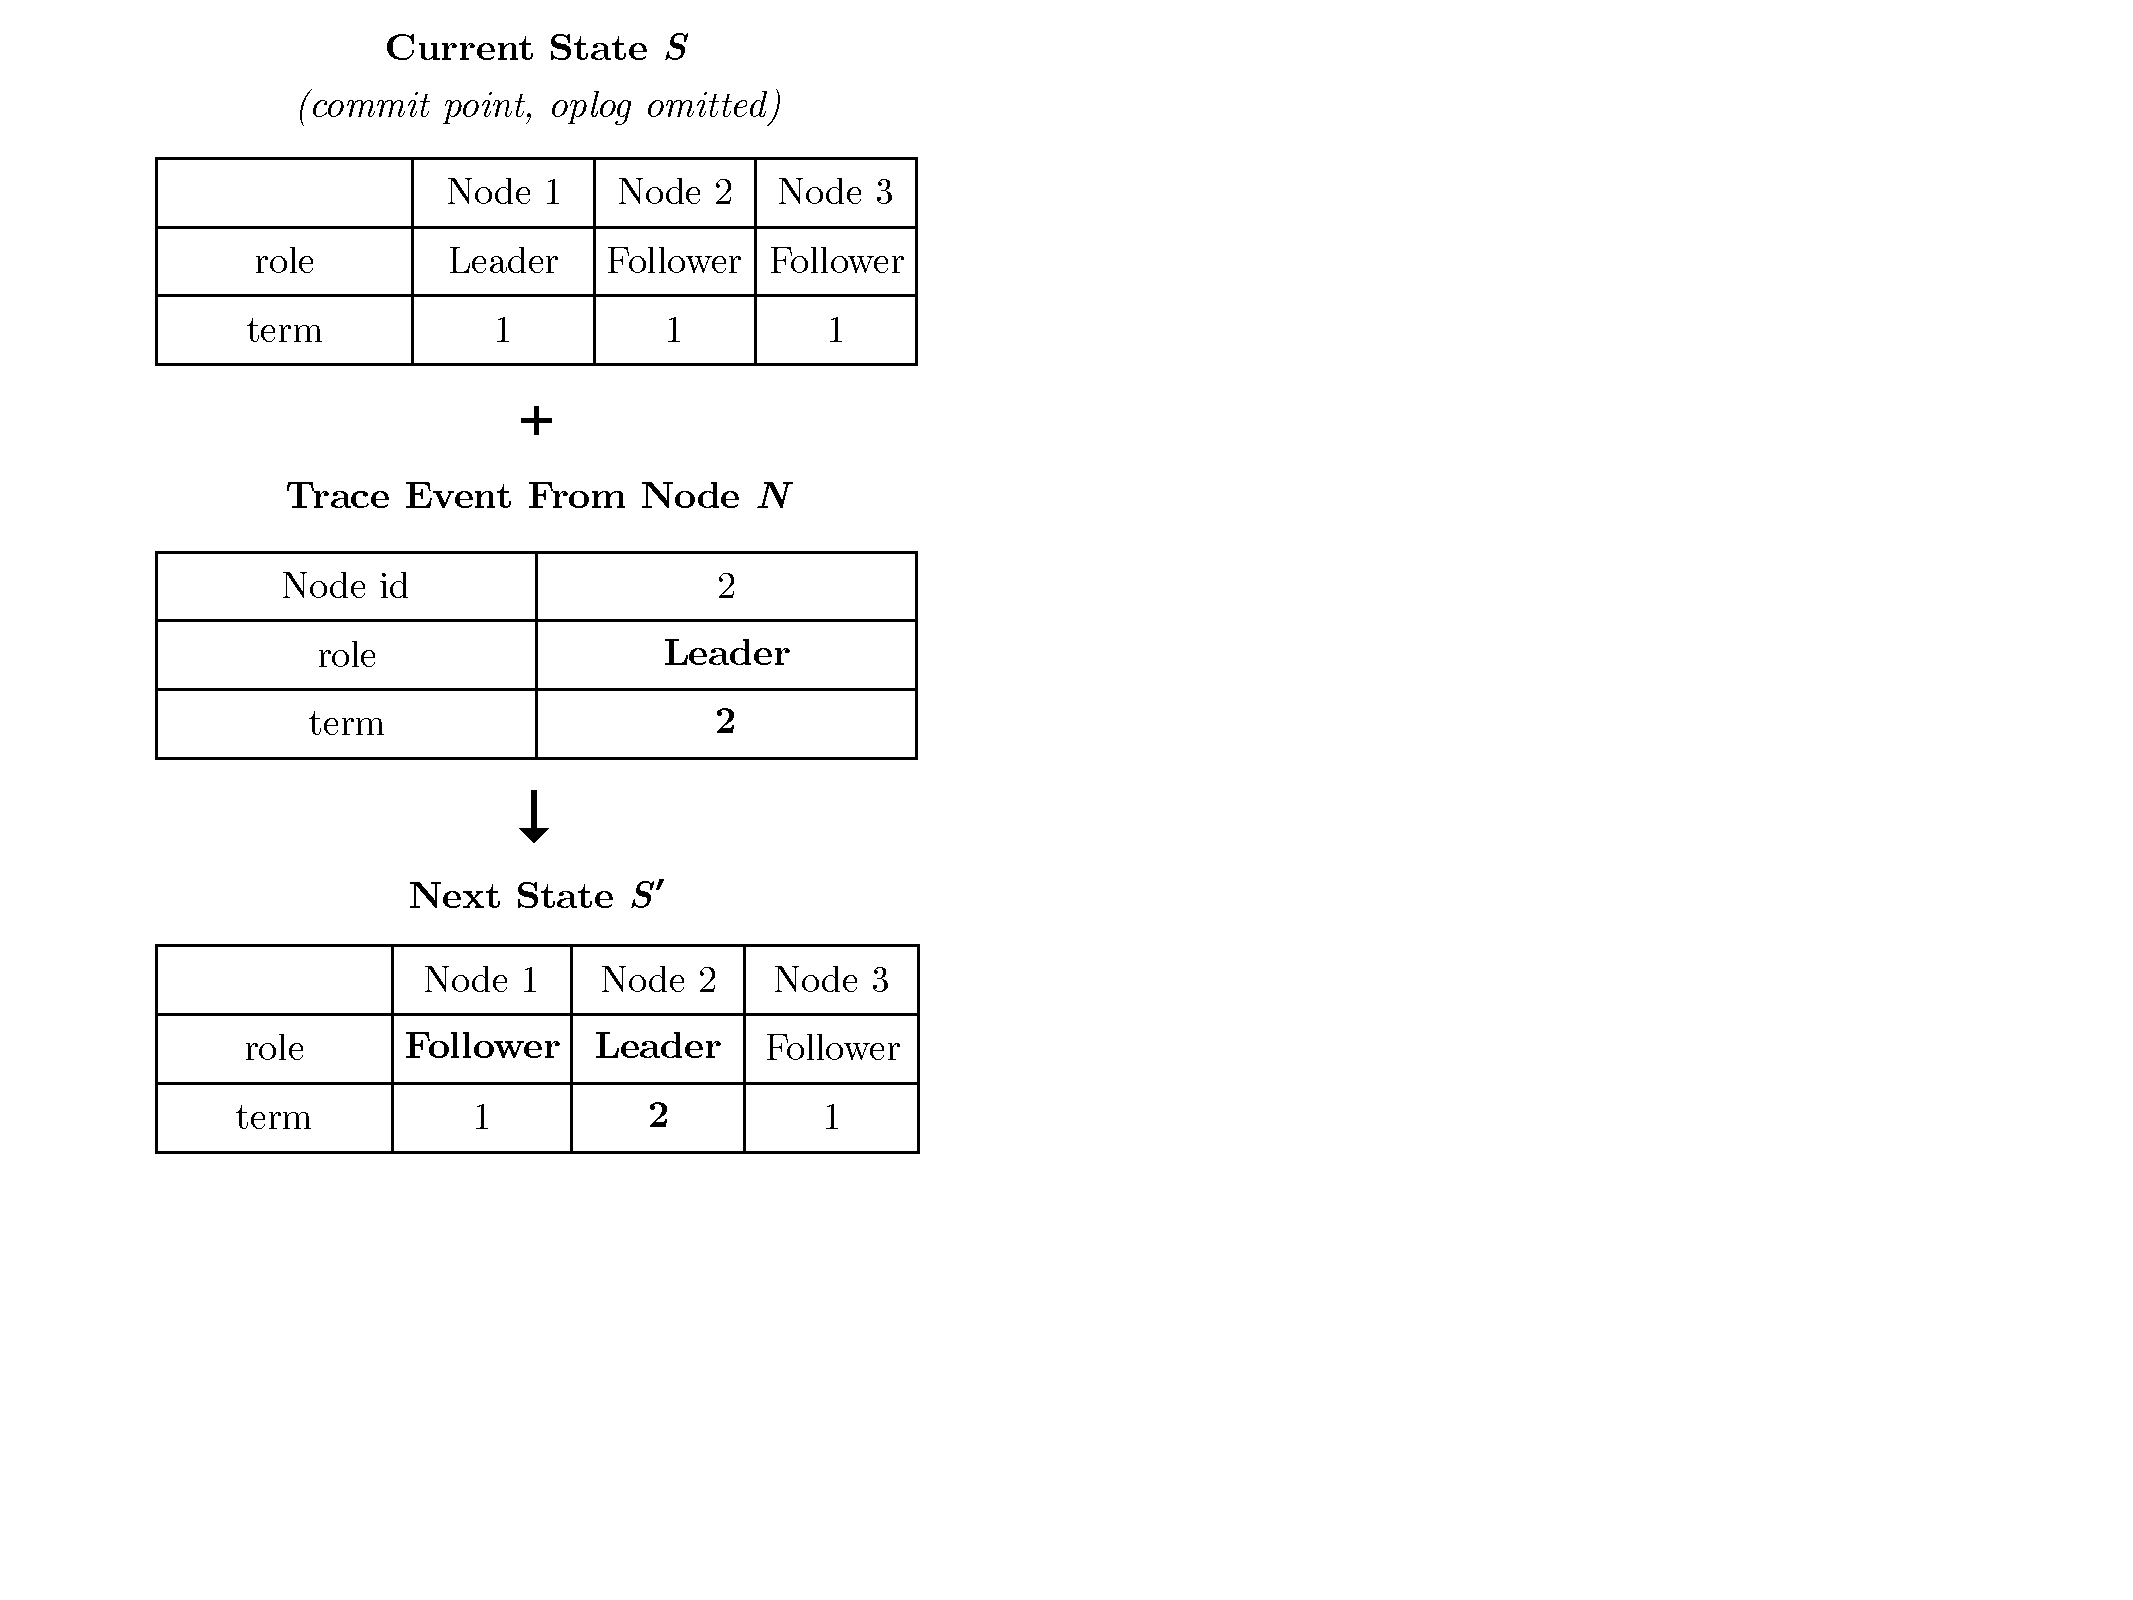
\includegraphics[width=\textwidth]{event-processing.pdf}
\caption{Trace Event Processing}
\label{figure:event-processing}
\end{figure}

Once the script constructs this sequence of states, it implements MBTC following a method proposed by Pressler \cite{Pressler18VerifyingSoftwareTracesTLAPlus}: it generates a TLA+ module called \texttt{Trace.tla} which includes the sequence of states (Figure \ref{fig:state-sequence}, a simplification from what our script actually produces), and uses the TLC model-checker to check that the sequence is permitted by the \texttt{RaftMongo.tla} model. The entire data pipeline can be seen in Figure \ref{figure:MBTC-pipline}. 
It was implemented by two engineers in two and a half months.

\begin{center}
\begin{tabular}{ | m{11em} | m{5em}| m{6em} | } 
\hline
Task & Effort & Lines of Code \\  
\hline
Event tracing & 4 weeks & 570 C++ \\ 
Update RaftMongo.tla & 3 weeks & 252 TLA+\\ 
Python post-processor & 3 weeks & 484 Python \\ 
\textbf{Total} & \textbf{10 weeks} & \\
\hline
\end{tabular}
\end{center}


\begin{figure}
\begin{verbatim}
------- MODULE Trace ------------
EXTENDS Integers, Sequences

\* Trace generated from replica set log files. Each
\* tuple is role, term, state, commit point, oplog
\* per node.

Trace == <<
<<
  <<"Leader", "Follower", "Follower">>,
  <<1, 1, 1>>,
  <<NULL, NULL, NULL>>,
  << <<>>, <<>>, <<>> >>
>>,
<<
  <<"Follower", "Leader", "Follower">>,
  <<1, 2, 1>>,
  <<NULL, NULL, NULL>>,
  << <<>>, <<>>, <<>> >>
>>
>>
\end{verbatim}
\caption{State sequence as TLA+ tuple (simplified)}
\label{fig:state-sequence}
\end{figure}

\begin{figure}
\begin{verbatim}
PROCEDURE becomeLeader() {
    acquire Lock A
    acquire Lock C
    role := Leader
    logTraceEvent()
}

PROCEDURE logTlaPlusTraceEvent() {
    /* Wrong acquisition order if called by
       becomeLeader, risks deadlock */
    acquire Lock A if not yet acquired
    acquire Lock B if not yet acquired
    acquire Lock C if not yet acquired
    read oplog
}
\end{verbatim}
\caption{Pseudocode for a replica becoming a Leader}
\label{fig:logTlaPlusTraceEvent}
\end{figure}

\subsection{Analysis}
\label{subsec:mbtc_analysis}

% Probably irrelevant: We considered either a Java harness that fed trace inputs to the TLC internal API, and we tried Pressler's method. Since the former was not fully implemented in Java for us, and the latter already works and includes nice Toolbox diagnostics, we stuck w/ the latter. We also considered Pressler's suggestion of using his method w/ a custom operator that avoids passing through TLA+ tuples as the repr of the trace, we didn't need to do that either.

% Counting from Oct 10, 2019 https://github.com/mongodb-labs/repl-trace-checker/commit/5c96b44d to 
% Jan 10+.
We had intended to trace-check several models against traces from both handwritten and fuzz tests, deploy the trace-checker to our continuous integration system, and measure accumulated state space coverage over all tests. 
Had we achieved this, we would have built much of the test infrastructure required for "eXtreme Modelling".
However, we applied trace-checking to only 5 handwritten tests and one fuzz test, \texttt{rollback\_fuzzer}. 
Only one handwritten test generated traces that passed the trace-checker. 
We did not deploy to continuous integration nor measure coverage. 
The effort to implement MBTC proved so costly for us that we abandoned the project after two and a half months of engineering effort. 

We faced complexities with concurrency and locking, discrepancies between our models and implementation, and incomplete support in TLC. 
In the following sections we describe these issues and propose future solutions.

\subsubsection{Visibility, hierarchical locking}
\label{subsubsec:mbtc_locking}

\textbf{Visibility}: When we began to add tracing to the MongoDB Server, we realized each trace event must be logged after it has occurred, but \textit{before} the change is visible to other replicas. 
E.g., when a leader receives a write from a client application and creates an oplog entry, it must log the \texttt{ClientWrite} event after the entry has appeared in its own oplog, but before any followers can replicate the entry and log an \texttt{AppendOplog} event for it. 
If a follower logged an \texttt{AppendOplog} event with an earlier timestamp than the leader's \texttt{ClientWrite} event, the trace would violate the causal relationship described in the model. 
To ensure each state change was logged before it became visible to other processes, our logging code had to hold one or more locks.

\textbf{Hierarchical locking}: Formal specifications of distributed systems algorithms, such as Raft, model a concurrent system of interacting processes, but they typically model each process as single-threaded. 
Production database systems such as the MongoDB Server, however, almost always have high intra-process concurrency and employ some degree of hierarchical locking \cite{Gray76SharedLocks}. 
The MongoDB Server specifically combines hierarchical locking with storage-engine Multi-Version Concurrency Control (MVCC), C++ latches, and higher level concurrency control primitives like futures.
It may not be feasible to log a consistent snapshot of such a process's state at the moment of a trace event.

% _tlaPlusRaftMongoEvent_inlock's caller has replcoord mutex, the fn gets Global IS,
% DB IS, and Collection IS locks for local.oplog.rs.
% more details in https://mongodbcr.appspot.com/536420002/, particularly patch set 9
% map locks A, B, C to RSTL, Global, replcoord mutex.

To implement MBTC for \texttt{RaftMongo.tla}, a replica must include the contents of its oplog with each trace event,
but acquiring the locks to obtain a snapshot of the oplog proved difficult. 
Suppose our \texttt{logTlaPlusTraceEvent} procedure (Figure \ref{fig:logTlaPlusTraceEvent}) must acquire locks A, B, and C, in that order, to read the oplog.
Consider a procedure \texttt{becomeLeader} that acquires locks A and C, then changes the replica's role to Leader. 
If we add a call from \texttt{becomeLeader} to \texttt{logTlaPlusTraceEvent}, the latter must acquire lock B, but this is the wrong order and risks deadlocking with other threads.
If \texttt{becomeLeader} first \textit{dropped} lock C, then acquired locks B and C, that would be the correct order.
But dropping lock C could allow a thread servicing an external request to communicate the node's new role to another process, thus making the role change \textit{visible} and violating the visibility rule described above.
General solutions are unpalatable: callers of \texttt{logTlaPlusTraceEvent} could be responsible for acquiring all the locks it will need, but this encodes intimate knowledge about \texttt{logTlaPlusTraceEvent} into its callers, and it significantly alters the system's behavior under test.

\begin{figure}
\begin{verbatim}
PROCEDURE becomeLeader() {
    acquire Lock A
    acquire Lock C
    role := Leader
    logTraceEvent()
}

PROCEDURE logTlaPlusTraceEvent() {
    /* Wrong acquisition order if called by
       becomeLeader, risks deadlock */
    acquire Lock A if not yet acquired
    acquire Lock B if not yet acquired
    acquire Lock C if not yet acquired
    read oplog
    /* Remainder of procedure as in Fig. 4 */
}
\end{verbatim}
\caption{Pseudocode for a replica becoming a Leader}
\label{fig:logTlaPlusTraceEvent}
\end{figure}

Solving both the visibility and the locking challenges, for each of the seven named state transitions in \texttt{RaftMongo.tla}, was the single most difficult aspect of our MBTC implementation, costing roughly a month of engineering effort. 
Eventually we discovered code locations that obeyed our visibility requirements, and we managed to avoid the need for acquiring locks out of order by exploiting MVCC features: it is possible with our storage engine to read from a snapshot of the oplog, instead of locking the oplog to read its most current contents.
Depending on which state transition was being traced, either reading from a snapshot was correct or locking the oplog was correct and did not risk deadlock.
Fortunately we discovered no cases where neither technique sufficed.

% Gravell: "3.3 Model-Based Trace-Checking
% To provide us with traces, we wrote a generic “trace bean” for capturing key transitions in a common database.
% Trace points were easily identified as a result of the close correspondence between top-level model and
% implementation. By hand we added trace beans and tracing code at each such point. Thereafter, each execution
% of the system automatically added to our tracing database. It was now easy to extract traces using SQL queries,
% and a small amount of scripting code, to extract and transform traces into forms that can be model-checked by
% Spin or ProB [14]."

In contrast to our difficulties adding tracing to the MongoDB Server, Gravell et. al. \cite{Gravell11ConcurrentDevelopmentOfModelAndImplementation} emphasize how easily they added tracing.
We believe their task was easier because 1) their application was a small prototype, 2) they had deliberately written their model and implementation to closely correspond (see Section \ref{subsubsec:modelling_for_trace_checking}), and 3) their application did not support the complex concurrency of a typical database.
We were surprised at the difficulty of adding tracing to the MongoDB Server, both because it had been easy for Gravell et. al. and because we had not anticipated how visibility and locking would complicate our code.
We expect any MBTC implementation for a concurrent database would encounter similar complexities with hierarchical locking and visibility of state changes.

\subsubsection{Implementation discrepancies}
\label{subsubsec:mbtc_impl_discrepencies}

The first discrepancy we found between our model and implementation involved MongoDB's concept of "arbiters".
MongoDB Server replicas can be configured as arbiters which vote in elections but have no data. 
\texttt{RaftMongo.tla} does not model arbiters and we did not implement tracing for them, thus tests which use arbiters failed when tracing was enabled.
This was trivial to understand and to ignore, but gave us a hint that our specs did not describe our implementation in as many cases as we wanted.

The second discrepancy was the behavior of \textit{initial sync}, the process a follower executes when it is added to the replica set in order to obtain a copy of the data and all oplog entries.
Trace checking the output of \texttt{rollback\_fuzzer} immediately reproduced a known violation \cite{SERVER-17934} of the specification: our implementation permits a new follower to acknowledge oplog entries as it receives them, before it is fully synced with the leader.
This behavior should not be permitted, because it leads to entries being considered majority-committed while part of the majority is still performing an initial sync.
We excluded this behavior from \texttt{RaftMongo.tla} when we first wrote it:
we did not have MBTC in mind, so we deliberately wrote an idealized model, with the intention to eventually bring our implementation into conformance.
When MBTC caught this violation it increased our confidence in trace-checking; however, it was not an acceptable outcome. 
Since the violation came only 4 steps from the trace's start, and the checker stopped at the first violation, the remainder of the 2,683 steps were unchecked. 

To permit \texttt{rollback\_fuzzer} to pass trace-checking, we could 1) fix the implementation sooner than planned, 2) avoid triggering the non-conforming behavior in testing, 3) update the model to match today's implementation, or 4) post-process the traces to simulate a conformant implementation.
Since this particular violation has minimum impact on users, we declined to fix it right away.
Instead we chose solution 2, and modified \texttt{rollback\_fuzzer} to ensure all followers were fully synced before the test began any writes. 

Other discrepancies required solution 3, updating the model. 
For example, \texttt{RaftMongo.tla} originally modeled the election term as a single global number known by all replicas.
This simplification was reasonable when the model was first written, since the election term was not the model's original focus. 
But in fact new election terms are gossiped among replicas, which each learn the new term at a different time.
MBTC required us to make the model more complex to match reality. 
We chose to update the model to resolve this and many other discrepancies: over the course of our research we added or changed 252 of the 345 lines of TLA+ in \texttt{RaftMongo.tla}, costing 3 weeks of effort.

In several cases we chose solution 4, post-processing the logs to simulate conformance. For example, in \texttt{RaftMongo.tla}, when a node performs an initial sync, it copies the leader's entire oplog.
In the implementation, a new node copies only recent entries.
The \texttt{RaftMongo.tla} behavior more closely matches the Raft protocol that inspired it, and makes it simpler to express invariants such as "an entry is committed after it is replicated to a majority of nodes' oplogs".
Making the implementation conform would discard a useful optimization, and updating the model would have required substantial effort.
Instead we resolved the discrepancy by adding logic to our Python script that filled in the missing entries while it generated the state sequence.
However, such an intrusive modification concerned us: a mistake in the Python script might mask a harmful transcription error in the database.
Given more time, we would have chosen solution 3, and updated the model to match the implementation.

Each discrepancy we discovered through MBTC required us to judge which of the four solutions to employ. 
Ideally, when an organization practices "eXtreme Modelling", they resolve each MBTC failure either by fixing the implementation or, if the failure is not a bug, by updating the model.
In practice, we often concluded it was better to work around violations instead of fixing them.
We chose to avoid the non-conforming behavior (solution 2) or to simulate a conformant behavior (solution 4) depending on which took less effort and least undermined our confidence in the test.
Unfortunately, our choices were based on estimates and guesses.
Such workarounds might not have been necessary if we began with a less abstract and idealized model, written for the purpose of MBTC.

\subsubsection{Modelling for trace-checking}
\label{subsubsec:modelling_for_trace_checking}

We tried to implement MBTC with models that had been written for a different purpose: for documenting and model-checking a design. 
We found that in order to use a formal model with MBTC, the model should be written with MBTC in mind.
If we began again, we would write our models to closely correspond to the implementation.
For example, we would name the operators and variables in the model after their counterparts in the implementation, the model's major components would be structured similarly to the implementation's, and critical sections of the implementation would correspond with single actions in the model.
In the case of multi-step events such as elections, we would model them with multiple actions, instead of expressing them as instantaneous single actions as we did in \texttt{RaftMongo.tla}.
We would faithfully model the flaws in the implementation if we did not plan to fix them immediately.

We would rewrite our specification to model events that are easily observed in the implementation: for example, we might model protocol messages, akin to the original Raft model.
We would try to avoid modelling state that is difficult to snapshot, especially if it were protected with complex locking.
If some state in the model cannot be logged by the implementation, Pressler proposes a "refinement mapping" technique \cite{Pressler18VerifyingSoftwareTracesTLAPlus} that is worth further investigation.

\subsubsection{Tooling and TLC}
\label{subsubsec:mbtc_tla_tlc}

Tool support for MBTC with TLA+ and TLC is a work in progress. 
Pressler's method worked well to check traces of hundreds of events, but for thousands of events it was impractically slow. 
Pressler proposed, and Markus Alexander Kuppe has begun to implement, features to check long traces by bypassing the TLA+ parser in favor of a special-purpose Java extension to TLC \cite{TLAPlusIssue413}. 
MBTC with TLA+ will be more convenient once these features are finalized and released, with publicly available examples. 
Another missing feature is the ability to combine state-space coverage reports over multiple TLC executions, which would permit engineers to calculate the total coverage achieved by deploying MBTC to continuous integration.

% what does MBTC prove?
% Advantage of MBTC over other tests is that implementation tests can't prove liveness, unless you run them forever. TLA+ specs can be checked for liveness, and if the impl matches the spec, the impl might also not have liveness bugs.

% impl is a subset of the spec => if the spec is safe, the impl is safe
% but we can't test to the point where we know that impl is a subset of the spec
% we only know that tested behavior is a subset of the spec

% FALSE: impl is a subset of the spec => if the spec has no liveness bugs, the impl has no liveness bugs
% the impl might lack spec behaviors that are required for liveness

% ********************************************************************
% ****************** MBTCG *******************************************
% ********************************************************************
\section{Model-Based Test-Case Generation}
\label{sec:model_based_test_case_generation}

TODO: This content can be added to this section or cut.
\subsection{Case Study: Realm mobile sync}
MongoDB Realm Sync requires an active-active replication protocol, and conflicts are resolved using Operational Transformation \cite{Stigsen19RealmPatent}.
The semantics of Operational Transformation are complex, and modelling them in TLA+ helped to both document and understand the desired decision tree.
Realm's mobile sync architecture requires implementing the Operational Transformation protocol in both C++ and Golang; the mobile database is written in C++ and the cloud sync server is written in Golang.
It is paramount that these two implementations resolve conflicts identically.
We improved our confidence that they do so by testing that they both conform to the model.

For this case study, we attempted a different technique: model-based test-case generation (MBTCG) \cite{Gravell11ConcurrentDevelopmentOfModelAndImplementation}.
We created unit tests for every state possible in the Operational Transformation spec and ensured that both the C++ and Golang implementations passed the unit tests.
These unit tests can be automatically generated and tested on any change to the model, and ensure that both implementations make appropriate changes to maintain equivalence. 
*****END Case Study: Realm mobile sync*****


% Outline of sections to follow: (doing them in this order tells the story of how the model-based testing happened chronologically and feels like the most natural way to split up the story)
% 1. Transcribed from C++ to TLA+. Ran the model checker, found issues.
% 2. C++ code generation, fine to mention stats of # test cases and lines of C++ code rather than in separate "Analysis" subsection.
% 3. Golang code generation. (this hasn't been implemented yet)

% TODO: We should double check with Drew D. what the name of the product and what the name of the team are (or at least what we're calling them externally).
MongoDB Realm Sync has 19 distinct operations which can be performed on a group of tables, an individual table, an object, or a list of values. These include operations such as deleting a table, creating a new object in a table, setting the property of an object, and inserting a new element into a list. Each type of operation must define how it merges with all other types of operations. This yields $19 (19 + 1) / 2 = 190$ merge rules needing to be defined with the remaining $19^2 - 190 = 171$ merge rules able to be inferred by symmetry. Approximately three-quarters of the merge rules have trivial implementations where the incoming operation is applied unchanged by both peers. The most complex merge rules are for the six array-based operations:

\begin{itemize}
  \item \texttt{ArraySet}: replacing the value of an existing element
  \item \texttt{ArrayInsert}: inserting a new element at a position within the list, or growing the size of the list by one
  \item \texttt{ArrayMove}: moving an element from one position to another
  \item \texttt{ArraySwap}: swapping the position of two elements
  \item \texttt{ArrayErase}: removing an element from the list
  \item \texttt{ArrayClear}: removing all of the elements from the list
\end{itemize}

% TODO: Do some LaTeX thing to make figure placement sane.
\begin{figure}
\begin{verbatim}
DEFINE_MERGE(ArrayErase, ArraySet)
{
  if (same_container(left_side, right_side)) {
    // LCOV_EXCL_STOP
    if (right_side.ndx == left_side.ndx) {
      // CONFLICT: Update of a removed element.
      //
      // RESOLUTION: Discard the UPDATE operation
      // received on the right side.
      right_side.discard();
    }
    else if (right_side.ndx > left_side.ndx) {
      right_side.ndx -= 1;
    }
    // LCOV_EXCL_START
  }
}
\end{verbatim}
\caption{C++ code for merging \texttt{ArrayErase} and \texttt{ArraySet} operations}
\label{fig:cpp_erase_set_merge}
\end{figure}

\subsection{Writing the TLA+ model}
\label{subsec:mbtcg_tlaplus}

MongoDB's Realm Sync Team wrote a TLA+ model for these array-based operations to assess the soundness of the existing C++ implementation and to provide a means for exhaustively generating test cases for a new Golang implementation. The $6 (6 + 1) / 2 = 21$ merge rules for the six array-based operations are implemented in approximately 1,000 lines of C++ code.

% Max likes the following phrase but it no longer has a sensible place to go.
% for conditionally adjusting the index numbers

% TODO: Do some LaTeX thing to make figure placement sane.
\begin{figure}
\begin{verbatim}
\* Returns a pair of sequences
\* <<server history, client history>> containing
\* the tails of serverLog and clientLog[c]
\* starting immediately after their common point
\* in history of when they were last merged
\* together.
Unmerged(c) ==
  Pair(SubSeq(serverLog,
              progress[c].serverVersion + 1,
              Len(serverLog)),
       SubSeq(clientLog[c],
              progress[c].clientVersion + 1,
              Len(clientLog[c])))

HaveUnmergedChangesOrAreConsistent ==
  \/ \E c \in Client :
        Unmerged(c) # Pair(<< >>, << >>)
  \/ \A c1, c2 \in Client :
        clientState[c1] = clientState[c2]
\end{verbatim}
\caption{TLA+ invariant for MongoDB Realm Sync}
\label{fig:tlaplus_realm_sync_invariant}
\end{figure}

Writing the TLA+ model took approximately 40 hours over the course of two weeks. The TLA+ model was written by copy-pasting the C++ code and then updating the syntax to be valid TLA+. The merge rule for two \texttt{ArrayInsert} operations was written first along with the \\ \texttt{HaveUnmergedChangesOrAreConsistent} invariant (see Figure \ref{fig:tlaplus_realm_sync_invariant}). The TLC model checker was run with constraints of 3 clients each performing a single operation on an array already containing 3 elements.
% TODO (Max): This still reads awkwardly to me and doesn't entirely capture the process. It may be necessary to describe what we did when a safety violation was found as it involved mostly tracing through the same steps of C++ code and mapping which branches to which set of nested IF and CASE statements we must have taken. Perhaps this is a good opportunity to reference what eXtreme Modelling brings up about the lack of good tooling?
The merge rules for a particular operation type were transcribed before running the TLC model checker. The merge rules for another operation type were only added after the TLC model checker found no safety violations.

This transcription process was challenging in two ways. First, the C++ code relies on mutable variables for expressing how the incoming operations must be modified to be correctly applied by the non-originating peer, whereas TLA+ variables cannot be mutated in the same way. Second, the order in which clients perform operations locally and then later merge with the server doesn't impact their final state, and, if left unconstrained, would quickly lead to a state space explosion.

% TODO: Do some LaTeX thing to make figure placement sane.
\begin{figure}
\begin{verbatim}
Transform_ArrayErase_ArraySet(left, right) ==
  CASE right.ndx = left.ndx ->
          \* Set the removed element.
          Pair(<<left>>, << >>)

    [] right.ndx > left.ndx ->
          \* Set an element after the position of
          \* the removed element.
          Pair(<<left>>,
               <<[right EXCEPT !.ndx = @ - 1]>>)

    [] OTHER -> Pair(<<left>>, <<right>>)
\end{verbatim}
\caption{TLA+ code for merging \texttt{ArrayErase} and \texttt{ArraySet} operations}
\label{fig:tlaplus_erase_set_merge}
\end{figure}

\subsubsection{Handling C++ mutability and flow control}

% TODO: Are there papers we could cite for these sort of challenges with TLA+?
TLA+ isn't a general-purpose programming language. \emph{Operators} in TLA+ (which behave most closely to a function in a general-purpose programming language) lack the concept of reassigning an argument or having a series of multiple \emph{expressions}. As shown in Figure \ref{fig:cpp_erase_set_merge}, the C++ variables \texttt{left\_side} and \texttt{right\_side} are mutated to produce the version of these operations to be applied on the non-originating peer. This mismatch between the two languages makes it more difficult to formalize a C++ source of truth into a TLA+ model, especially in the presence of nested if-statements. Additionally, a series of multiple if-statements must be transcribed to explicitly define all branch combinations that may or may not be taken consecutively. Fortunately, the TLC model checker was readily able to catch human transcription errors as safety violations. Some examples of transcription errors were forgetting to substitute the updated index number in later comparisons, or entirely forgetting to embed a deeply-nested or later occurring if-statement as another nested \texttt{CASE} statement.

\subsubsection{Constraining the state space}

In addition to transcribing from C++ to TLA+ being a time-intensive process, verifying the TLA+ with the TLC model checker was itself a time-intensive process---at least until the state space was artificially constrained. One simplification made during the conception of the TLA+ model was to have a \texttt{MergeAction} which simultaneously uploads any changes from the client and downloads any changes from the server. Having these be distinct actions within the TLA+ model would only have been beneficial when explicitly modelling time. Instead, the TLA+ model is being used to generate C++ and Golang test cases where clients perform a sequence of operations starting from the same initial array. A client performing a sequence of operations that are causally dependent on another client's sequence of operations is equivalent to the first client performing its sequence of operations on a different initial array. Since the TLC model checker explores all clients performing all sequences of operations, a sufficiently large initial array should cover TODO (Max) "all cases" what to say here.

We artificially constrained the state space to have clients perform and merge operations in ascending order of their id to avoid exploring redundant states. We aren't able to define the clients as a symmetry set because the client id is used as the discriminator for which happens later when the timestamps for the operations are equal. The specification doesn't model time at all so client 2's operation always happens after client 1's though not every merge rule will consider the timestamp as the operations are also based on the same version of the array. This means that using 3 clients covers both the case (for client 2) of merging with an earlier operation (from client 1) and a later operation (from client 3).

\subsubsection{Results from the TLC model checker}

In addition to detecting safety violations caused by transcription errors, the TLC model checker also encountered a \texttt{StackOverflowError} due to a case in the merge rule for the \texttt{ArraySwap} and \texttt{ArrayMove} operations leading the merge function to never terminate. This issue was found to also exist in the C++ code; the bug had faithfully been transcribed from C++ to TLA+. It was surprising to discover a bug in the C++ implementation due to the maturity of the product and the amount of randomized testing that had gone into it. To work around the bug, the \texttt{ArraySwap} operation excluded from testing for the remainder of this experiment.

The TLC model checker not finding a violation of the \texttt{HaveUnmergedChangesOrAreConsistent} invariant doesn't say anything about the model describing what the C++ implementation actually does. A trivial way to achieve convergence (at the cost of user-intent preservation) would be to have every merge rule clear the contents of the array. We still need to test that the behavior of the model conforms to the C++ code.

\subsection{Generating C++ test cases}
\label{subsec:mbtcg_cpp}

The state space explored by the TLC model checker provides an exhaustive set of test cases for how a given pair of operations should be transformed when applied by the non-originating peer. The TLC model checker supports writing the graph of all reachable states as a DOT file. The \texttt{-dump dot,actionlabels graph} option causes the TLC model checker to generate a graph.dot file where nodes in the graph are labeled with the state (a conjunction of assignments to all \texttt{VARIABLE}s declared in the TLA+ specification) and edges are labeled with the action taken to progress from one state to the next.

A BNF grammar for the output of \texttt{TLCStateMut\#toString()} was written and a parser generator for Golang was used \cite{GoccGitHub} to generate a parser for it. The state graph for a run with 3 clients each performing a single operation was then analyzed in a Golang program to generate C++ test cases composed of (1) the initial array, (2) the operations each client performed, and (3) the transformed version of the operations each client applied after merging the original operations from the other clients. The Golang program then produces a C++ program which uses MongoDB Realm Sync's unit test framework. The \texttt{fixture.sync\_all\_clients()} call takes the place of performing the merge action for all the clients (in the same order the TLA+ model performs the merge).

\begin{figure}
\begin{verbatim}
TEST(Transform_Node__6971023528664242108)
{
  size_t num_clients = 2;
  TransformArrayFixture fixture{
    test_context, num_clients, {1, 2, 3}};

  fixture.transaction(0, [](TableRef array) {
    array->set_int(0, 2, 4);
  });
  fixture.transaction(1, [](TableRef array) {
    array->remove(1);
  });

  fixture.sync_all_clients();
  fixture.check_array({1, 4});

  fixture.check_instrs(0, {ArrayErase{1}});
  fixture.check_instrs(1, {ArraySet{1, 4}});
}
\end{verbatim}
\caption{C++ test case for merging \texttt{ArrayErase} and \texttt{ArraySet} operations}
\label{fig:cpp_test_erase_set_merge}
\end{figure}

% 4913 test cases with 3 element array, 3 clients performing 1 operation each
% 50653 test cases with 5 element array, 3 clients performing 1 operation each
For an initial array containing 3 elements and 3 clients each performing a single operations, the Golang program generated 4,913 C++ test cases. The existing C++ unit tests for the merge rules of the array-based operations covered 18 of 86 branches (21\%). The generated C++ unit tests covered all 86 of 86 branches (100\%). The coverage of the specific sections of the C++ code was measured by adding in \texttt{LCOV\_EXCL\_STOP} and \texttt{LCOV\_EXCL\_START} comments within the block of the \texttt{same\_container()} condition. This is because the TLA+ model was designed to only exercise cases where the clients are acting on the same array.

% TODO (Max): We should potentially describe a change made in the TLA+ model to make it more useful at the expense of not exactly representing what the C++ code does.
% Elements within a list are referred to by their index number. The array-based operations make up ~1,000 lines of C++ code of conditionally adjusting index numbers to define 6 * (6 + 1) / 2 = 21 merge rules.

The initial array is all that is required to vary in order to generalize the operational transform algorithm. Using three clients handles the cases where the ``left'' merges with a ``right'' operation which happens earlier in time (client 2 integrating client 1's changes) and the ``left'' merges with a ``right'' operation which happens later in time (client 3 integrating client 1's and client 2's changes). All states explored are covered by a different initial array which could be reached by the first operation of one client and some other operation representing its transform across the first operation. TODO Need to mention something about this being for the clients performing more than a single operation each, and why we only need 3 array elements.

TODO: Add in the diagram that we drew

TODO (Max)

% ********************************************************************
% ****************** Conclusions *************************************
% ********************************************************************
\section{Conclusions}
\label{sec:conclusions}

We suspect that MBTCG succeeded for MongoDB Realm Sync and MBTC failed for the MongoDB Server primarily due to code size. 
The implementation associated with the TLA+ model for Realm Sync was a few hundred lines of code. 
The MongoDB Server is hundreds of thousands of lines of code; the replication protocol alone is tens of thousands of lines.
Realm Sync's spec was also deliberately written with a close correspondence to the implementation, whereas the MongoDB Server's spec was written as a highly simplified abstraction of one aspect of the replication protocol.
The close correspondence of the former was key to Realm Sync's success, however any close correspondence with the MongoDB Server's implementation would inevitably have made the spec overly complicated for its purpose, and likely it would have inflated the state space beyond what is feasible to model-check.
In the absence of a close correspondence, MBTCG seems unfathomable and MBTC requires significant post-processing of traces. 
We learned that in a system of the MongoDB Server's size and complexity, post-processing is unavoidable, and should be used early and often.
The definition of a "trace event" must be loosened, to only include readily available state, and then post-processing can fill in the unavailable state, that presumably hasn't changed since a different action event.
This may mask some bugs, and it is critical to think about which bugs the MBTC effort is aimed at catching and which ones other testing will cover.
MBTC in a system of the Server's scale will likely require a significant investment for every single spec, and an initial infrastructure investment will not be sufficient.

MBTC and MBTCG are both promising approaches to ensuring conformance between a spec and an implementation.
In a small system, MBTCG was highly effective and accomplished its goal. When MBTCG is possible, and when the state space is not too large, MBTCG is the gold standard of ensuring model-implementation conformance.
If the state space becomes too large though, we must start sampling the space, and MBTC can be a good way to do that.
MBTC is also a good approach when it can be difficult to create unit tests for modelled behavior.
However, when the implementation becomes too large, neither may be possible without a large investment per-model.

Future work should make both model-based testing approaches more practical.
TLC performance was an obstacle, and any improvements would be highly valuable.
Better research and tooling to post-process partial states and merge them together under certain assumptions could make the post-processing safer and easier.
More research should determine best practices for writing models intended to be used in model-based testing.
It should also determine best practices for logging trace events and generating test-cases from a model.
Developing tooling for whole-process snapshotting could have greatly simplified MBTC trace logging, since we could have just used the snapshots to create trace events.
Making MBTC and MBTCG first-class features in TLC could have saved us a great deal of time.


%\end{document}  % This is where a 'short' article might terminate

% ensure same length columns on last page (might need two subsequent latex runs)
\balance
% ********************************************************************
% ****************** Acknowledgements ********************************
% ********************************************************************
%ACKNOWLEDGMENTS are optional
\section{Acknowledgments}
\label{sec:acknowledgments}
Many experts have advised us, proposed workarounds for obstacles, reviewed our code, and reviewed drafts of this paper, including 
David Bradford,
Mark Callaghan,
Mike O'Brien,
Siyuan Zhou,
Will Schultz,
Michael Cahill,
Tess Avitabile,
Henrik Edin,
Andy Schwerin,
and Ron Pressler.
We are embarrassingly indebted to Markus Alexander Kuppe for answering our questions about TLC within minutes, and implementing features we requested within hours.

% The following two commands are all you need in the
% initial runs of your .tex file to
% produce the bibliography for the citations in your paper.
\bibliographystyle{abbrv-original-case}
\bibliography{main}  % use main.bib file
% You must have a proper ".bib" file
%  and remember to run:
% latex bibtex latex latex
% to resolve all references
\end{document}
\balance
